\chapter{Deviation of $\Tmn$ from equilibrium in Au+Au collisions at $\Elab$ = 5--160 \emph{A} GeV}
\label{chap:local_equilibration}

The importance to quantify the deviation of the local energy-momentum tensor from
equilibrium is discussed in \ref{sec:fluidization}. This quantification allows to assess
the uncertainty arising from neglecting the non-equilibrium part of $\Tmn$ at
fluidization, an approximation adopted by most of the existing approaches (see section
\ref{Sec_II} for details).

Therefore, the following questions are addressed here for Au+Au collisions
at $\Elab = $ 5--160 \emph{A} GeV, varying the collision centrality and nuisance
parameters:

\begin{itemize}
    \item How far away are $\Tmn$ and $\jmu$ from the ideal fluid form at the time of
          geometrical overlap --- typical fluidization time in many approaches?
          %Equations (\ref{EqI}-\ref{EqII}) are used to quantify the deviations.
    \item What are the main sources of deviation from equilibrium? 
    \item Is there a better fluidization criterion? Should it depend on centrality?
\end{itemize}

\section{Methodology to quantify off-equilibrium contributions in $\Tmn$ and $\jmu$} \label{sec:Methodology}

The calculation is based on the hadronic transport approach called
Ultra-relativistic Quantum Molecular Dynamics (UrQMD 3.4)
\cite{Bass:1998ca,Bleicher:1999xi}, which is similar to the SMASH transport
approach described in detail in chapter \ref{chap:smash} . The degrees of
freedom in UrQMD are hadrons, resonances up to a mass of 2.2 GeV and strings
and the implemented processes include binary elastic and inelastic scatterings
which mainly proceed via resonance formation and decays or string excitation
and fragmentation at higher collision energies. The UrQMD particles move along
classical trajectories and scatter according to their free-particle
cross-sections. In this study  no long range potentials are employed and
particle trajectories between collisions are always straight lines. Using UrQMD
Au + Au collisions at laboratory frame energies $\Elab =$ 5, 10, 20, 40, 80 and
160 \emph{A} GeV are simulated.

The general procedure for the calculations is:
\begin{enumerate}
\item Generate many UrQMD events and coarse-grain them using a 2+1D space-time
  grid. The space dimensions are chosen to be the event plane xz. A 2+1D grid
  and not 3+1D is chosen, because observing the behaviour of some quantity on a 2D
  surface versus time is much easier and informative for a human than observing
  a quantity on a 3D grid.  Additionally, in central collisions due to symmetry the
  event plane completely characterizes all the volume. The center of mass frame
  is used as the computational frame in the simulation.  In all the following
  text the time is measured in the center of mass frame.  By the UrQMD convention
  $t = 0$ is the moment when the contracted spheres of the nuclear radius first
  touch each other in a central collision.
\item Particles from the generated events are used to construct the
  energy-momentum tensor $\Tmn(t,x,z)$ locally for each grid cell as described in
  section \ref{sec:final_coarse_graining}. To compute $\Tmn$ only participants
  are taken into account, i.e. the particles that took part in at least one
  collision.
\item Transform the constructed energy-momentum tensor in each grid cell to the
  Landau rest frame according to Eq. (\ref{eq:lrf}).
\item Verify the weak conditions given by Eqn. (\ref{cond_to_check})
  locally in time and space. The conditions for smallness of pressure
  anisotropy, off-diagonality, Eckart velocity relative to Landau are tested. The
  condition for smallness of bulk pressure compared to pressure is ignored, because
  it depends on the equation of state, which can be different for different
  models that use fluidization.
\end{enumerate}

This procedure is nothing but the fluidization of hybrid models with the
additional quantification of the deviations from equilibrium.

\section{Sensitivity to statistics, grid spacing and smearing}\label{Sec_V}

Before showing the final results, in this section the influence of nuisance
parameters is investigated. Let us first consider the influence of the number
of Monte-Carlo events used to produce $\Tmn$ and $\jmu$.

The deviations of $\Tmn$ in the simulation from the ideal fluid $\Tmn_{ideal}$
can have two distinct reasons. The first one is the deviation of the
distribution function $\mathit{f}(\vec{r},\vec{p})$ in the transport approach
from equilibrium, this reason is referred to as physical. The second reason is
statistical: due to finite number of particles in the simulation, the
distribution function is not sampled exactly.

Let us consider two energy-momentum tensors: calculated from particles
$\Tmn_{part}$ and a ''true'' $\Tmn$:

\begin{align}
  \Tmn_{part}(\vec{r}) =\frac{1}{N_{ev}} \sum_{events} \sum_i \frac{p^{\mu}_i p^{\nu}_i}{p^0_i} K(\vec{r} - \vec{r_i}, p_i) \\
  \Tmn(\vec{r}) = \int \frac{p^{\mu} p^{\nu}}{p^0} \mathit{f}(\vec{r},\vec{p}) d^3p
\end{align}

Here $N_{ev}$ is the number of events and $K(\vec{r} - \vec{r_i}, p_i)$ is a
smearing kernel. The particular form of the kernel is discussed in section
\ref{sec:tmn_wavepacket}. In the limit of $N_{ev} \to \infty$

\begin{align}
  \frac{1}{N_{ev}} \sum_{events} \sum_i K(\vec{r} - \vec{r_i}, p_i) \xrightarrow{N_{ev} \to \infty} \\ \int d^3p \, d^3r' \, \mathit{f}(\vec{r'}, \vec{p}) K(\vec{r} - \vec{r'}) \nonumber
\end{align}

For the case of a Gaussian kernel and $\sigma \to 0$, the kernel turns into a
$\delta$-function and one retains the ''true'' $\Tmn$. To combine
these two limits ($\sigma \to 0$, $N_{ev} \to \infty$) one has to keep enough
particles within a volume of size $\sigma^3$. Consequently, to obtain the
''true'' $\Tmn$ in the simulation, one has to take the limit ($\rho$ is the particle
number density)

\begin{align} \label{Eq:true_Tmn_condition}
  \sigma \to 0,\, N_{ev} \, \rho \, \sigma^3 \to \infty
\end{align}

\begin{figure}
  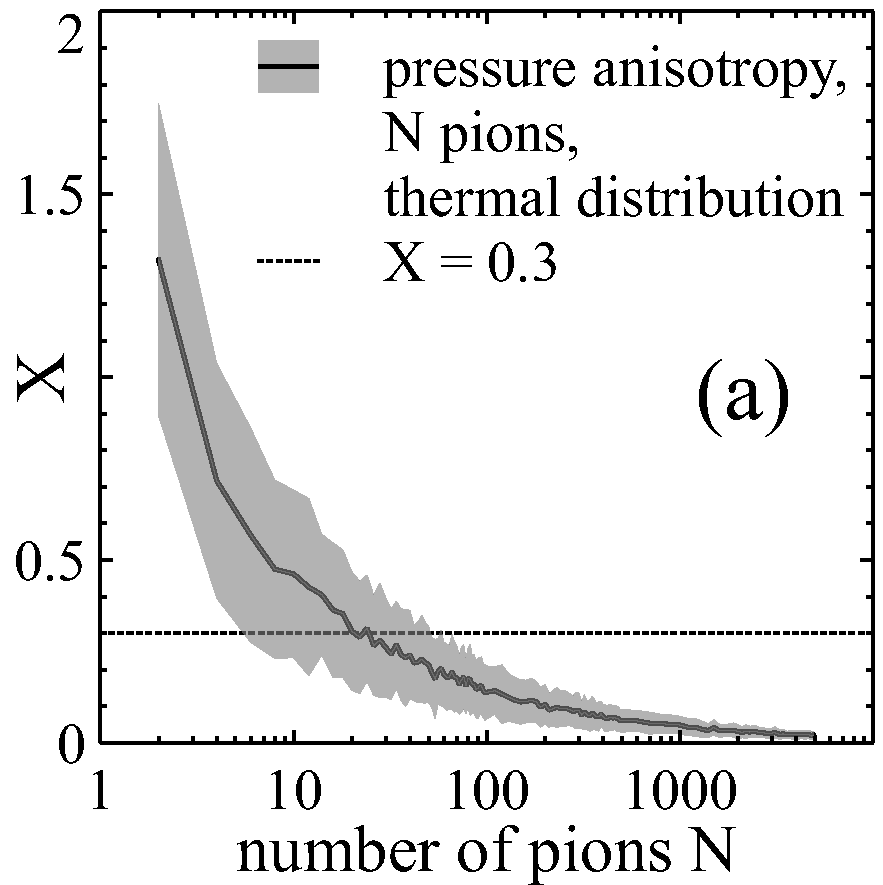
\includegraphics[width = 0.49\textwidth]{plots/thermalization_urqmd/x_pure_stat.pdf}
  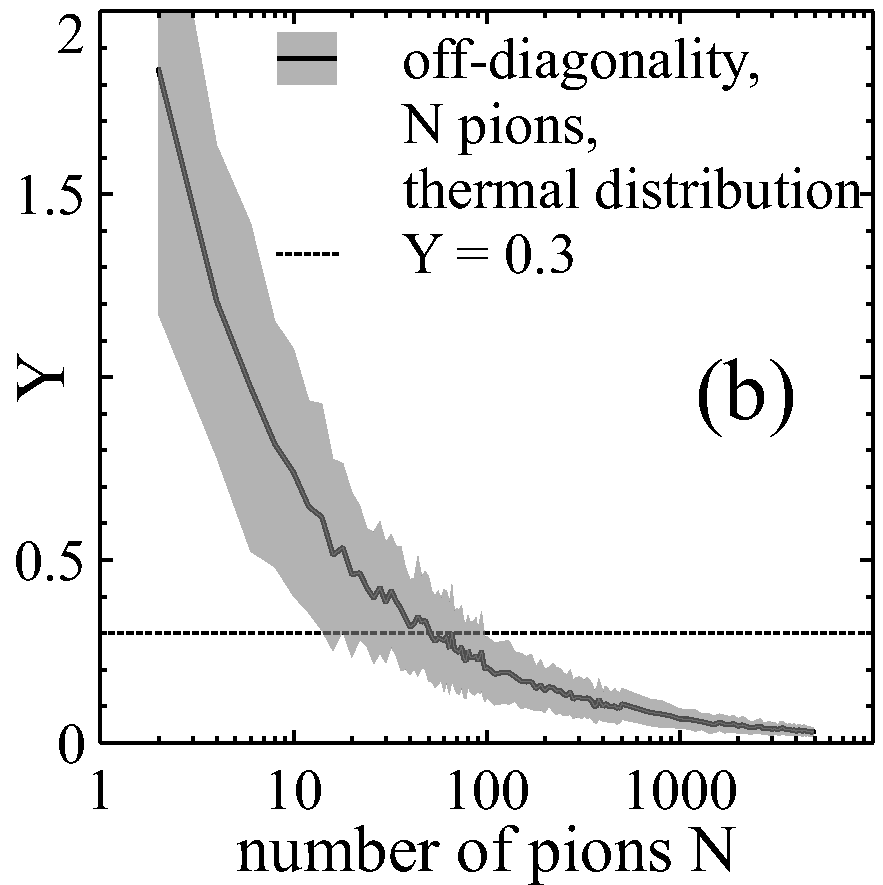
\includegraphics[width = 0.49\textwidth]{plots/thermalization_urqmd/y_pure_stat.pdf}
  \caption{Pressure anisotropy $X$ (panel a) and off-diagonality $Y$ (panel b)
  of $\Tmn$ for particles sampled according to thermal distributions. The effect
  of statistics on the deviation of energy-momentum tensor from the ideal fluid
  one is demonstrated.}
  \label{FIG:pure_stat_effect}
\end{figure}

This creates practical limitations for determining the ''true'' $\Tmn$ in
simulations: decreasing $\sigma$ by a factor of 10 demands increasing the statistics
by a factor of 1000! Also see regions with lower density are more demanding
with respect to statistics. To get some insights into the effect of statistics, 
an auxiliary simulation is performed: $N$ pions are generated, their momenta being
sampled from a thermal distribution with an ad-hoc temperature of $T = 0.2$ GeV,
then $\sum \frac{p^{\mu} p^{\mu}}{p^0}$ is computed, pressure isotropy $X$ and
off-diagonality $Y$ of the energy-momentum tensor from Eq. (\ref{cond_to_check})
are calculated. The number of pions $N$ was varied and $X$ and $Y$ are plotted versus
$N$. The results can be seen in Fig. \ref{FIG:pure_stat_effect}. For every point
the simulation was repeated 100 times and the standard deviation is displayed as
an error. For the thermal distribution $X=Y=0$ in the limit of $N\to \infty$, so
Fig. \ref{FIG:pure_stat_effect} demonstrates a pure effect of sampling a finite
number of particles.

Fig. \ref{FIG:pure_stat_effect} can be used to specify the number of events
needed to reach a good enough approximation to the ''true'' $\Tmn$. For example,
for $Y=0.3$ as an acceptable level, the condition of Eqn.
\ref{Eq:true_Tmn_condition} becomes $N_{ev} \rho \sigma^3 > 100$. From Fig.
\ref{FIG:pure_stat_effect} one can also see that the off-diagonality $Y$ is more
sensitive to statistics than the pressure isotropy $X$.

In the previous paragraph the effect of statistics itself was considered rather
as an obstacle to get the physical ''true'' $\Tmn$. However, recently
event-by-event simulations gained popularity, where the initial state for
hydrodynamics is intentionally constructed from a small number of events to
include the fluctuations. Let us see, how the number of events influences
deviations of $\Tmn$ from the ideal form in heavy ion collisions. The $\Tmn$ was
computed locally on every point of the grid, and as a general characteristic
the percentage of the event-plane area is chosen, where $X < 0.3$ ($Y < 0.3$). To
define the total area numerically, only grid cells, where pressure $p > 10^{-4}$
GeV/fm$^3$ are taken into account. For this example Au+Au collisions at $E =
80\emph{A}$ GeV with the impact parameter $b = 6$ fm are considered. The
smearing parameter $\sigma$ is 0.8 fm. Results are depicted in
Fig.~\ref{FIG:sensitivity_Nev}.

\begin{figure}
  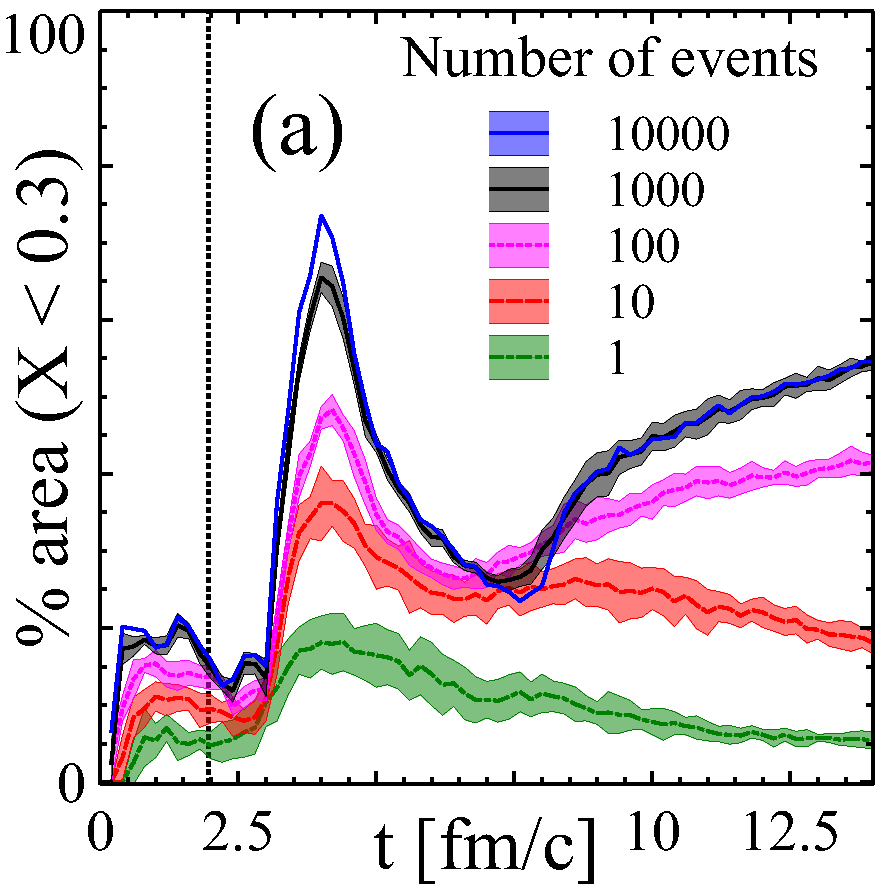
\includegraphics[width = 0.49\textwidth]{plots/thermalization_urqmd/E80_b6_x_area_Nev_dep.pdf}
  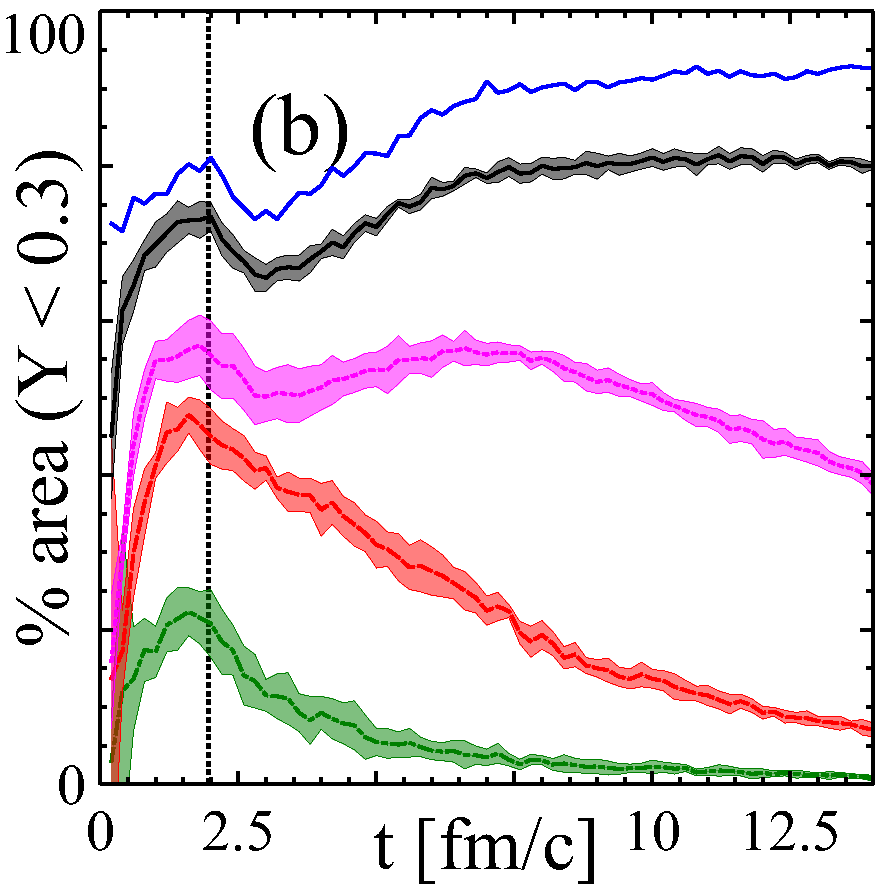
\includegraphics[width = 0.49\textwidth]{plots/thermalization_urqmd/E80_b6_y_area_Nev_dep.pdf}
  \caption{Event plane area percentage, where the pressure isotropy $X$ (panel a) or
           off-diagonality $Y$ (panel b) does not exceed 0.3 versus time for different
           number of events $N_{ev}$ used to construct $\Tmn$. Number of events
           $N_{ev} = 1$ corresponds to the event-by event case. The dotted line marks
           the geometrical overlap time.}
  \label{FIG:sensitivity_Nev}
\end{figure}

\begin{figure}
  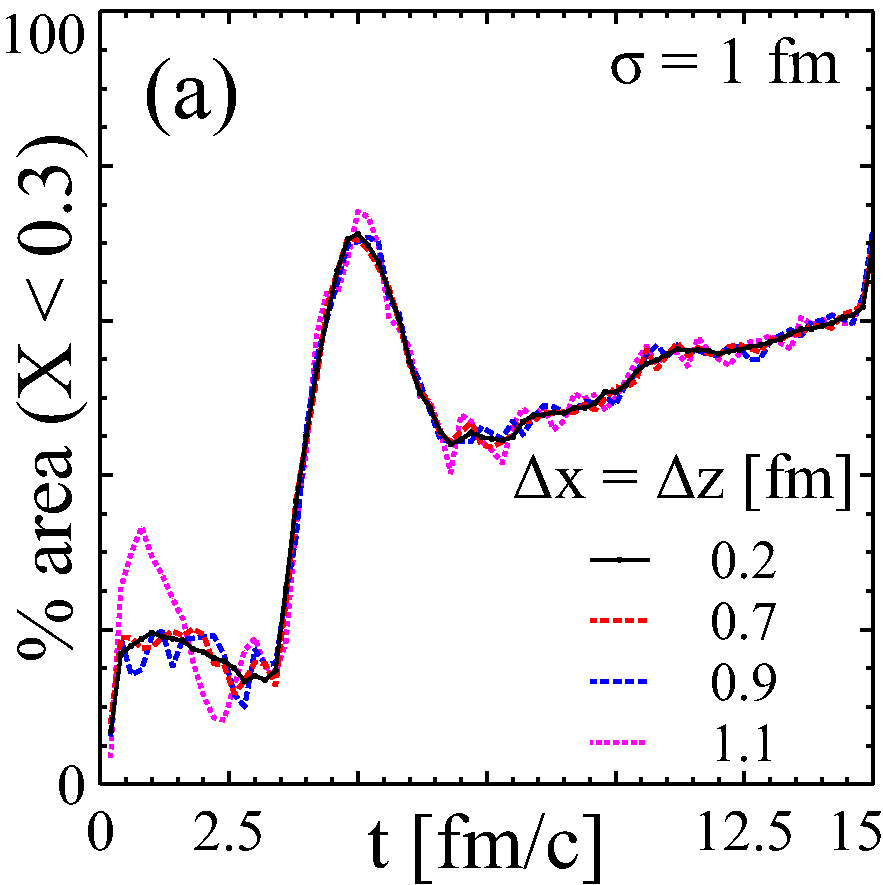
\includegraphics[width = 0.49\textwidth]{plots/thermalization_urqmd/grid_size_sensitivity.pdf}
  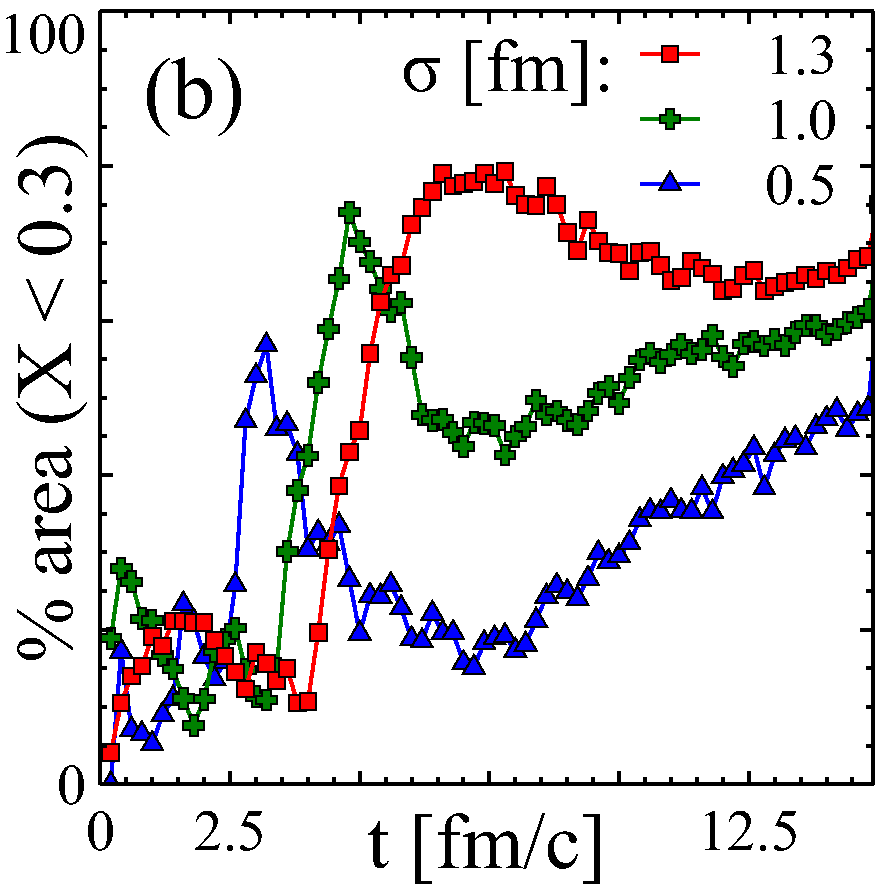
\includegraphics[width = 0.49\textwidth]{plots/thermalization_urqmd/sigma_sensitivity.pdf}
  \caption{Event plane area percentage, where pressure isotropy $X$ does not
           exceed 0.3. Au+Au versus time. $E = 80\emph{A}$ GeV, centrality $b = 6$ fm,
           number of events $N_{ev} = 1000$. Gaussian smearing $\sigma$ (right) and grid
           spacing $\Delta x = \Delta z$ (left) are varied to study sensitivity of results
           to them.}
  \label{FIG:sensitivity_sigma_dx}
\end{figure}

One can see that for this given $\sigma$ 1000 events are enough for $X$ to
saturate, so the line for $N_{ev} = 1000$ represents results for the physical
pressure isotropy, i.e. due to deviation of $\mathit{f}(\vec{r},\vec{p})$ in the
transport from equilibrium. For $Y$ at $N_{ev} = 10000$ almost all the event
area has small off-diagonality, which means that the physical off-diagonality is
small. For event-by-event simulations deviations of $\Tmn$ from ideal fluid are
dominated by statistical effects.

In addition to the effect of statistics the effect of other nuisance parameters
was investigated, i.e. the grid spacing and the Gaussian smearing. According to
Fig.~\ref{FIG:sensitivity_sigma_dx}, the grid spacing does not influence the
results, if taken sufficiently small. This is expected, because the grid does
not participate in the simulation or in the calculation of $\Tmn$, it only
determines the resolution of the $\Tmn$ output. The only effect of the grid spacing
is on the precision of the area calculation by counting cells, here the resolution
of the output matters. At early times, it makes some difference, because the
total area is small. That is why in the following $\Delta x = \Delta z = 0.6$
fm was chosen. At the same time the Gaussian width $\sigma$ influences the results very
significantly, as it can be seen from Fig.~\ref{FIG:sensitivity_sigma_dx}. The
effect of $\sigma$ is twofold: on the one hand a larger $\sigma$ means
effective increase of statistics. On the other hand, if the pressure anisotropy
is large at some space point due to physics, the Gaussian smearing will spread
this asymmetry in a 1-2 $\sigma$ radius.

\begin{figure}
  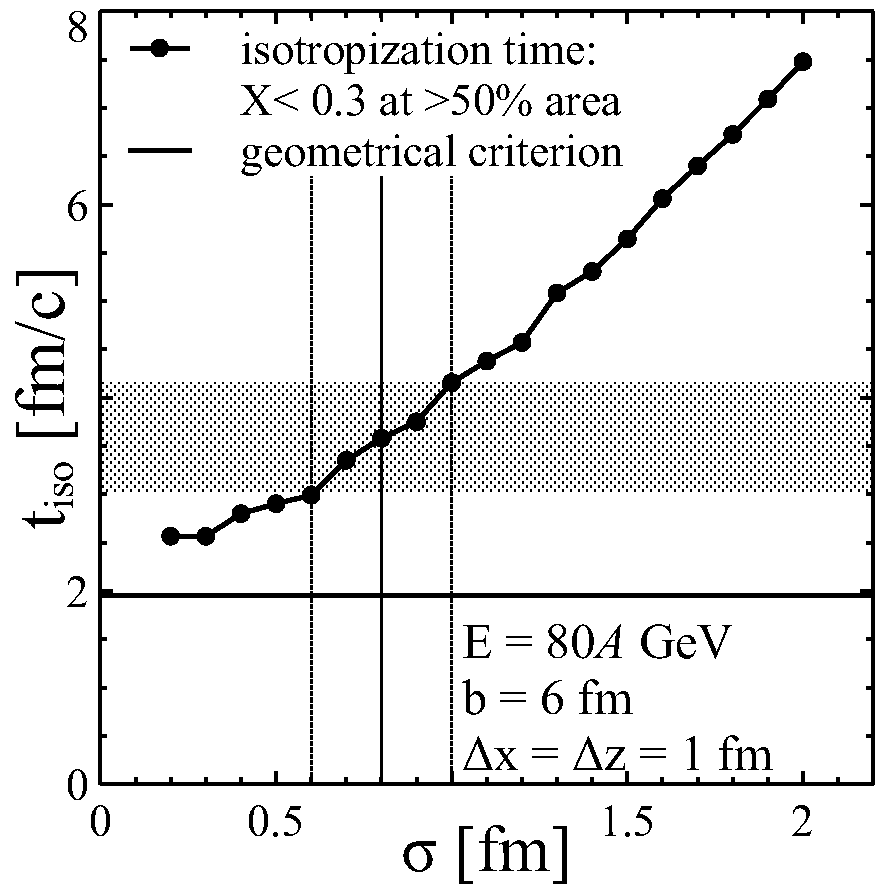
\includegraphics[height = 9cm]{plots/thermalization_urqmd/t_iso_vs_sigma.pdf}
  \caption{Isotropization time (such time that more than 50\% of event plane
           area have pressure isotropy $X < 0.3$) versus $\sigma$.}
  \label{FIG:t_iso_sensitivity_sigma}
\end{figure}

To characterize the influence of $\sigma$ in a simpler way, $t_{iso}$ versus
$\sigma$ was plotted, where $t_{iso}$ is the earliest time when at least 50\%
of the area have $X < 0.3$. Let us refer to this time as \emph{isotropization time}
as it is further described in the following Section. In
Fig.~\ref{FIG:t_iso_sensitivity_sigma} this dependence is displayed, the
isotropization time is monotonously growing with $\sigma$ and is approaching
the geometrical time for~$\sigma \to 0$. Taking the limit $\sigma \to 0$ is
computationally challenging, because one has to increase statistics as
$\sigma^{-3}$, as shown previously. Instead a reasonable value $\sigma = 0.8$
fm was chosen and systematic errors were assigned to our results, corresponding
to changing $\sigma$ in the range $(0.6-1.0)$ fm. Another justification for
this treatment is that none of the existing models attempts to consider the
''physical'' limit of $\sigma \to 0,\, N_{ev} \rho \sigma^3 \to \infty$, all
the models use some fixed width instead.

\section{Results} \label{sec:Results}

\begin{figure*}
  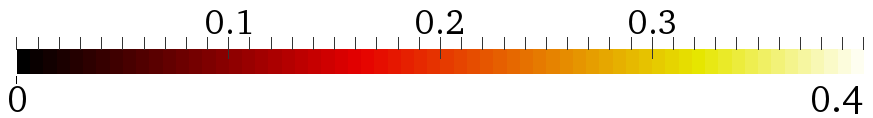
\includegraphics[height = 1cm]{plots/thermalization_urqmd/E80b6_x_paraview_color_legend.png} \\
  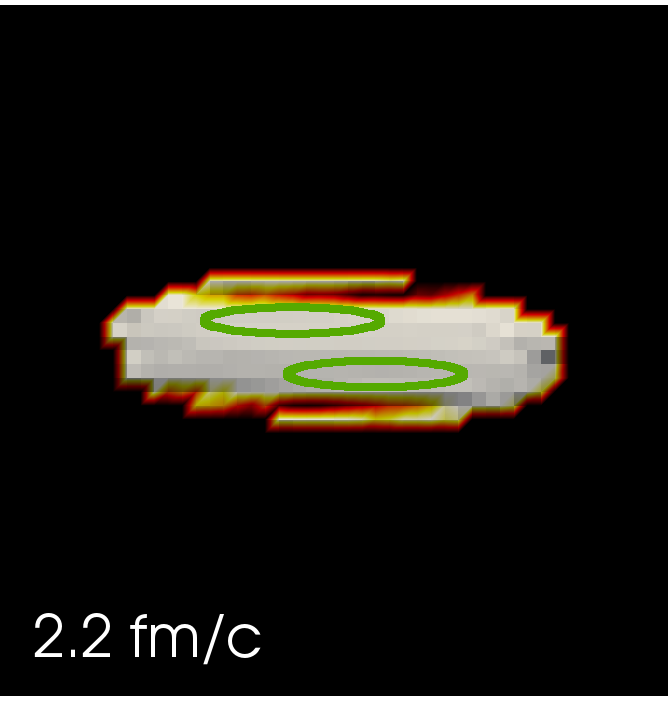
\includegraphics[width = 3.0cm]{plots/thermalization_urqmd/E80b6_x_paraview_t2_2fm.png}
  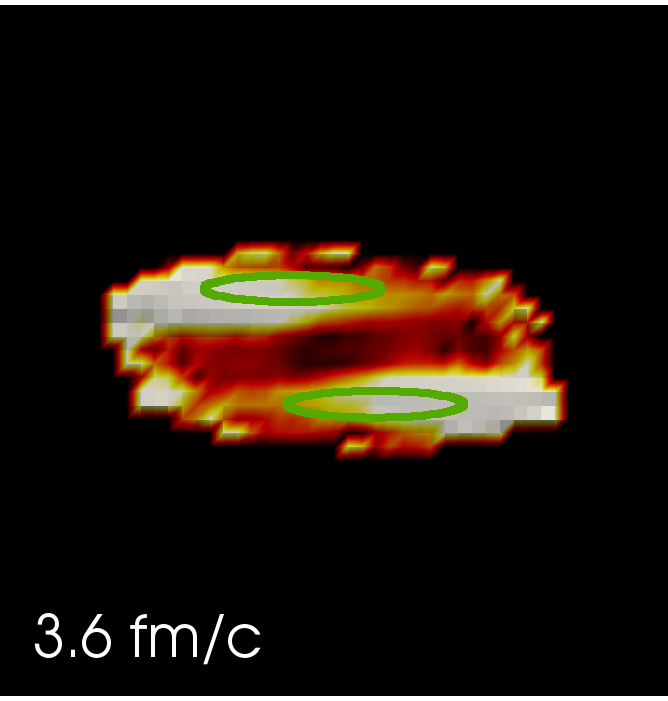
\includegraphics[width = 3.0cm]{plots/thermalization_urqmd/E80b6_x_paraview_t3_6fm.png}
  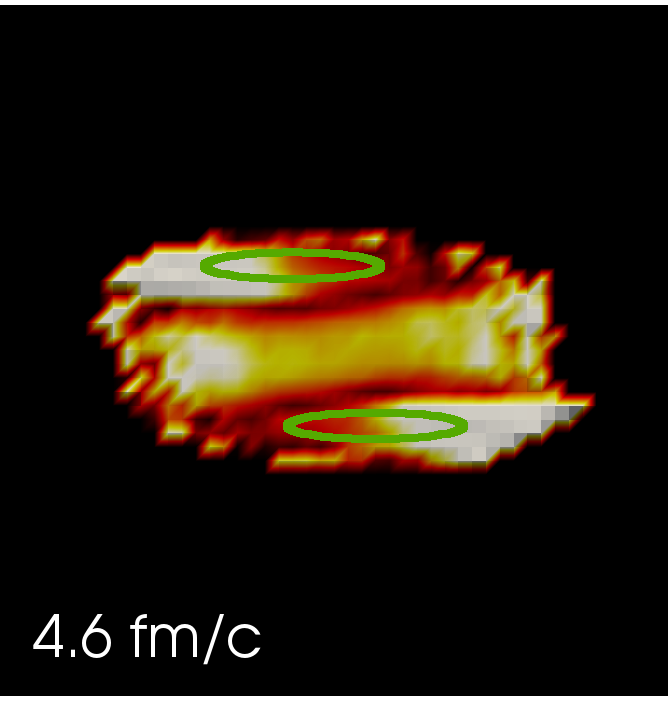
\includegraphics[width = 3.0cm]{plots/thermalization_urqmd/E80b6_x_paraview_t4_6fm.png}
  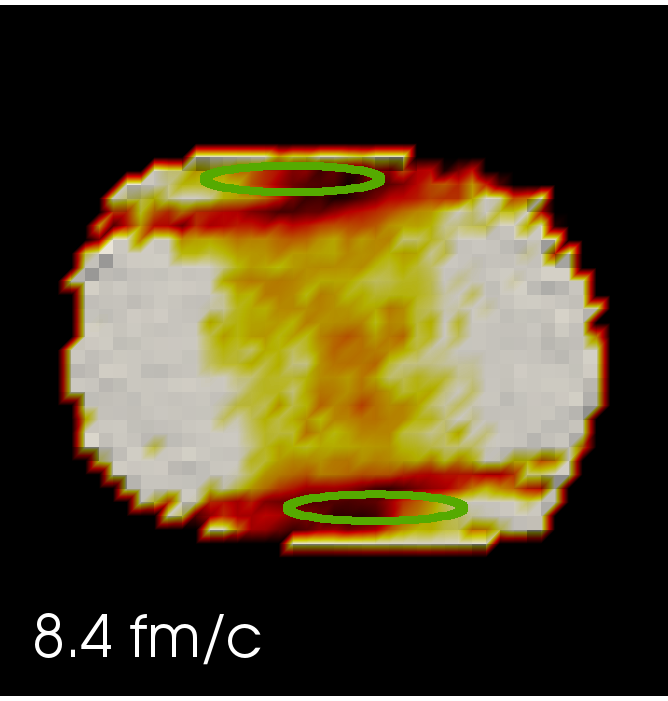
\includegraphics[width = 3.0cm]{plots/thermalization_urqmd/E80b6_x_paraview_t8_4fm.png}
  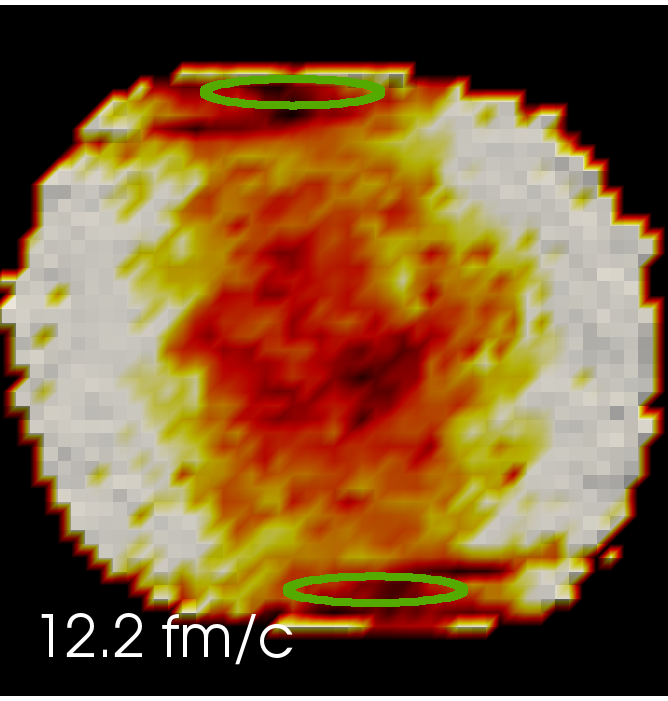
\includegraphics[width = 3.0cm]{plots/thermalization_urqmd/E80b6_x_paraview_t12_2fm.png}
  \caption{Space-time evolution of the pressure anisotropy $X =
           \frac{|T_L^{11}-T_L^{22}|+|T_L^{22}-T_L^{33}|+|T_L^{33}-T_L^{11}|}
           {T_L^{11}+T_L^{22}+T_L^{33}}$
           (see color scale above the Fig.) for collision energy
           $\Elab = 80$ \emph{A} GeV and impact parameter $b = 6$ fm.
           If the value of $X$ exceeds color map maximum, it is marked with the same
           color as maximum. Solid lines mark the positions of the nuclei, if they
           would not interact.}
  \label{FIG:x_paraview_space_time_evolution}
\end{figure*}

While in the previous section the effects of nuisance parameters on
the energy-momentum tensor generated from particles were studied, here the
dependence on physical parameters is considered, namely collision energy and centrality.
All the following figures are shown for grid spacing $\Delta x = \Delta z = 0.6$ fm,
Gaussian smearing $\sigma = 0.8$ fm, and number of events $N_{ev} = 1000$.
The smearing kernel is defined as in section \ref{sec:final_coarse_graining}.

\subsection{Pressure anisotropy}

\begin{figure}
  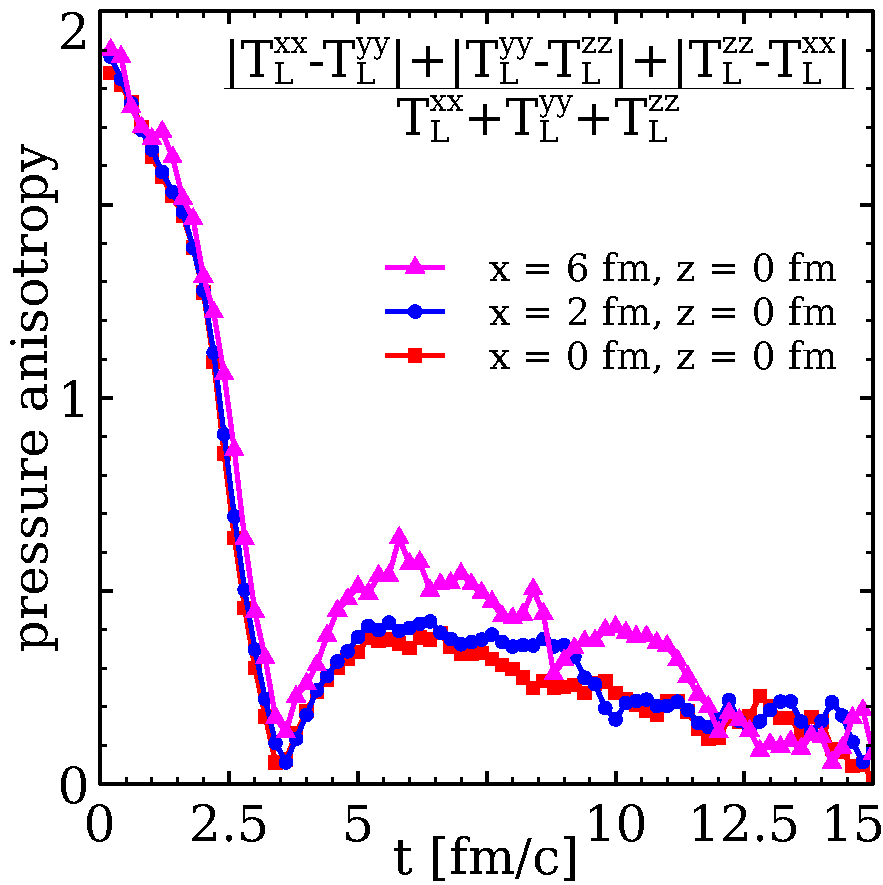
\includegraphics[width = 7cm]{plots/thermalization_urqmd/E80b6_x_vs_t_few_space_points.pdf}
  \caption{Example for the behaviour of the pressure anisotropy versus time in Au+Au
           collisions at $\Elab = 80$ \emph{A} GeV and impact parameter $b = 6$ fm.}
  \label{FIG:x_vs_t_few_space_points}
\end{figure}

The pressure anisotropy $X$ satisfies the following properties: $X \le 2$ for
any tensor and $X = 0$, if and only if $T^{11}_L = T^{22}_L = T^{33}_L$ as it is
for an ideal fluid. For viscous hydrodynamics it is necessary that $X \ll
1$. Here $X_{crit} = 0.3$ is considered as a limiting value, when viscous
hydrodynamics is still applicable. Changing $X_{crit}$ to 0.4 leaves one with
qualitatively the same results and conclusions. Fig.
\ref{FIG:x_paraview_space_time_evolution} gives a qualitative impression of the
space-time evolution of the pressure anisotropy. Even though the figure shows a
particular energy of $\Elab = 80\emph{A}$ GeV and centrality $b = 6$ fm, some
features are universal for all energies and centralities that were considered:

\begin{itemize}
  \item On the borders of the expanding system the anisotropy is always high,
        thus these regions are never consistent with viscous hydrodynamics.
  \item After some moment of time a relatively isotropized central region
        rapidly expands and never disappears completely during the time evolution
\end{itemize}

To make quantitative statements let us consider the evolution of the pressure
anisotropy at several points along the x axis (z = 0) versus time. This is shown
in Fig.~\ref{FIG:x_vs_t_few_space_points}. One can see that in the beginning the
anisotropy is almost maximal, then it rapidly decreases and never rises too much
again. As shown in the previous section, $N_{ev} = 1000$ is enough to
suppress the anisotropy due to statistics, so the behaviour of $X$ in
Fig.~\ref{FIG:x_vs_t_few_space_points} is dominated by physics. However, the
impact of statistical fluctuations can be observed already at $t > 5$ fm/c: $X$
starts to fluctuate in space and time. One can see this both in
Fig.~\ref{FIG:x_paraview_space_time_evolution} at later times and in
Fig.~\ref{FIG:x_vs_t_few_space_points}.

\begin{figure}
  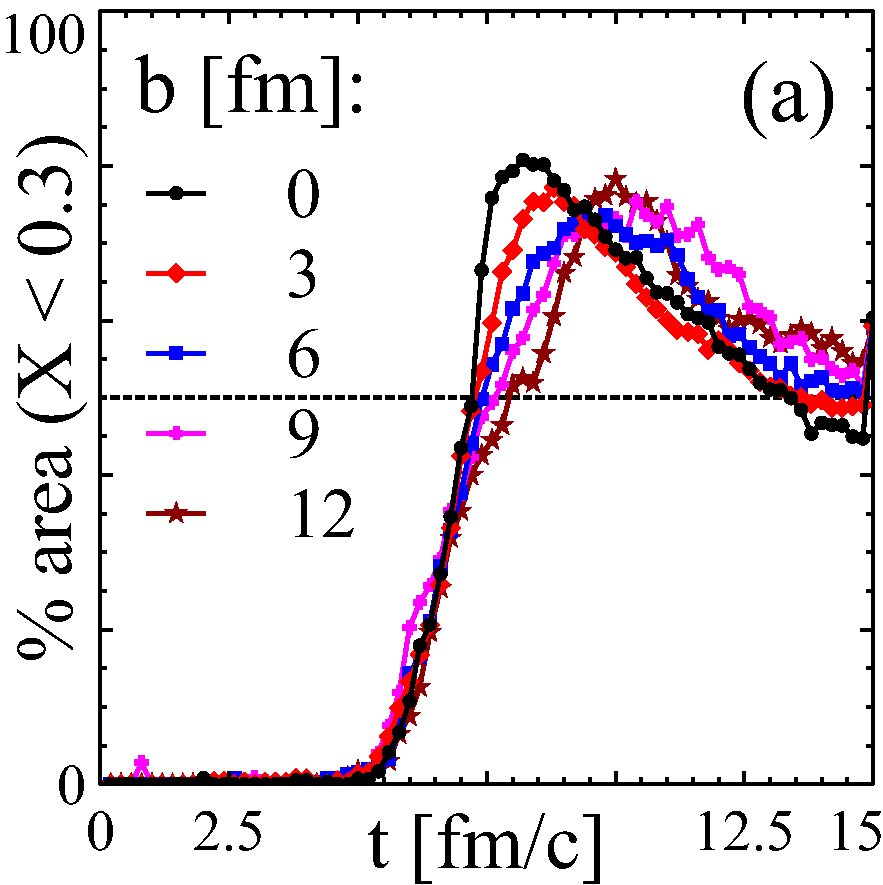
\includegraphics[width = 0.32\textwidth]{plots/thermalization_urqmd/plot_x_area_percentages_E5.pdf}
  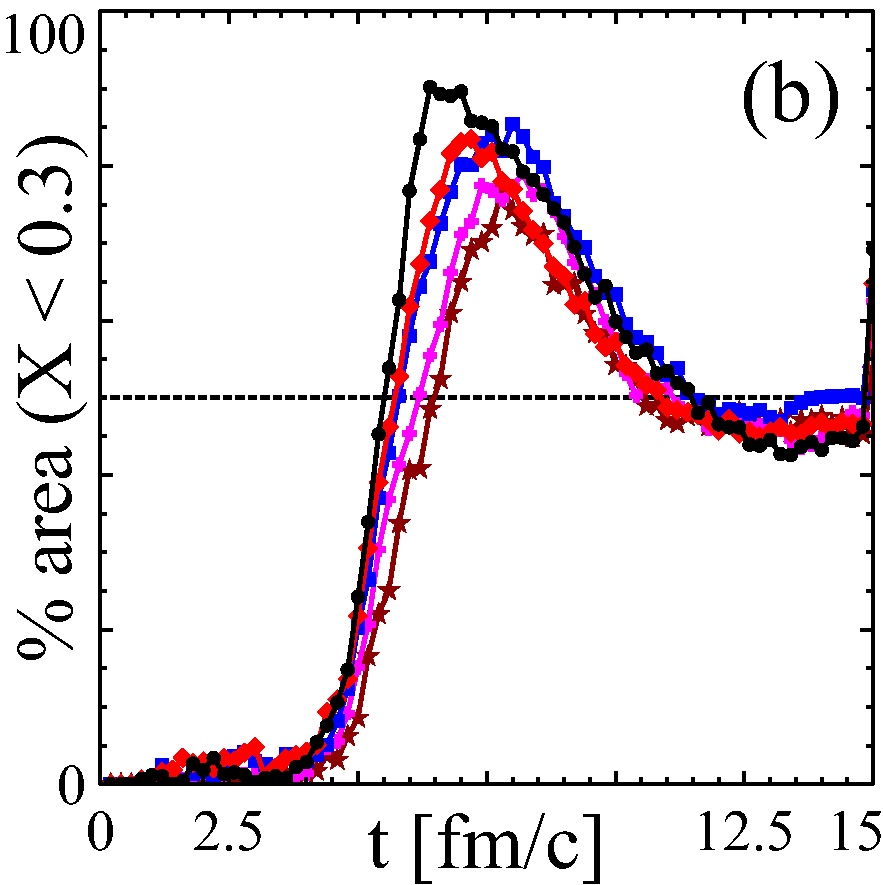
\includegraphics[width = 0.32\textwidth]{plots/thermalization_urqmd/plot_x_area_percentages_E10.pdf}
  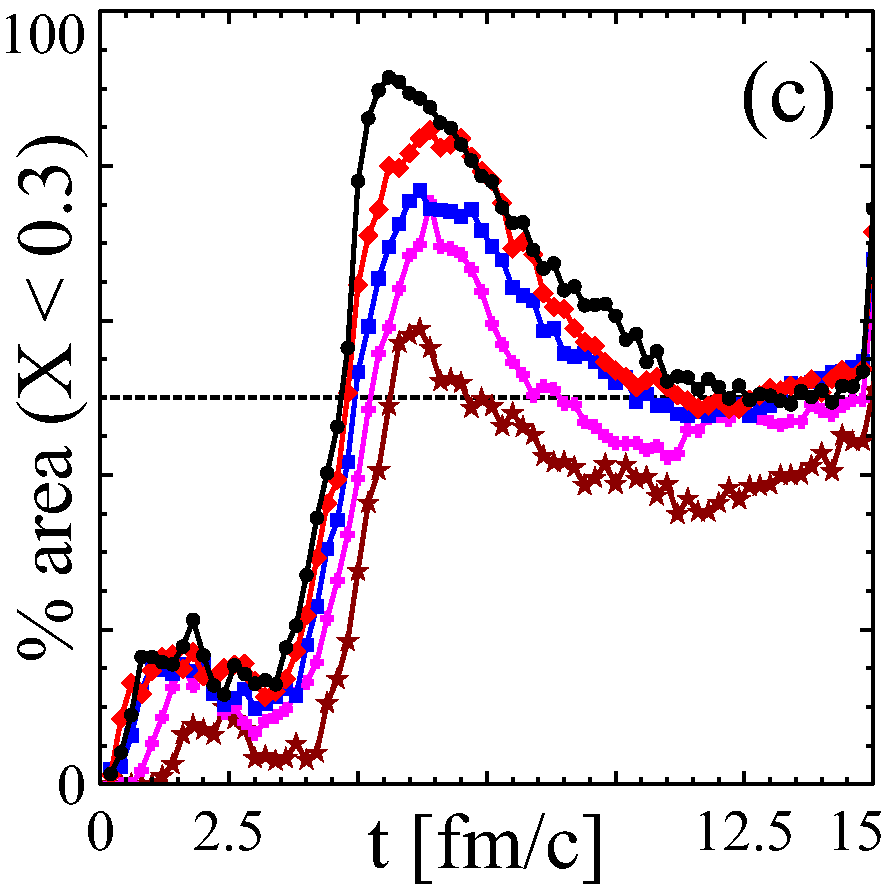
\includegraphics[width = 0.32\textwidth]{plots/thermalization_urqmd/plot_x_area_percentages_E20.pdf}\\
  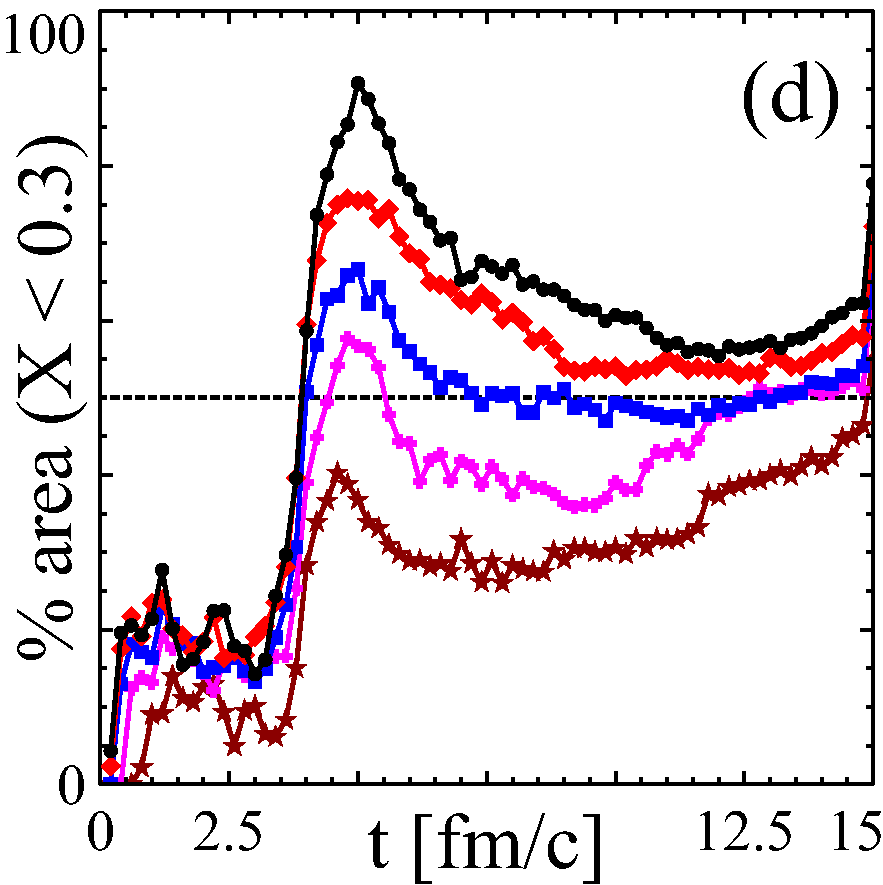
\includegraphics[width = 0.32\textwidth]{plots/thermalization_urqmd/plot_x_area_percentages_E40.pdf} 
  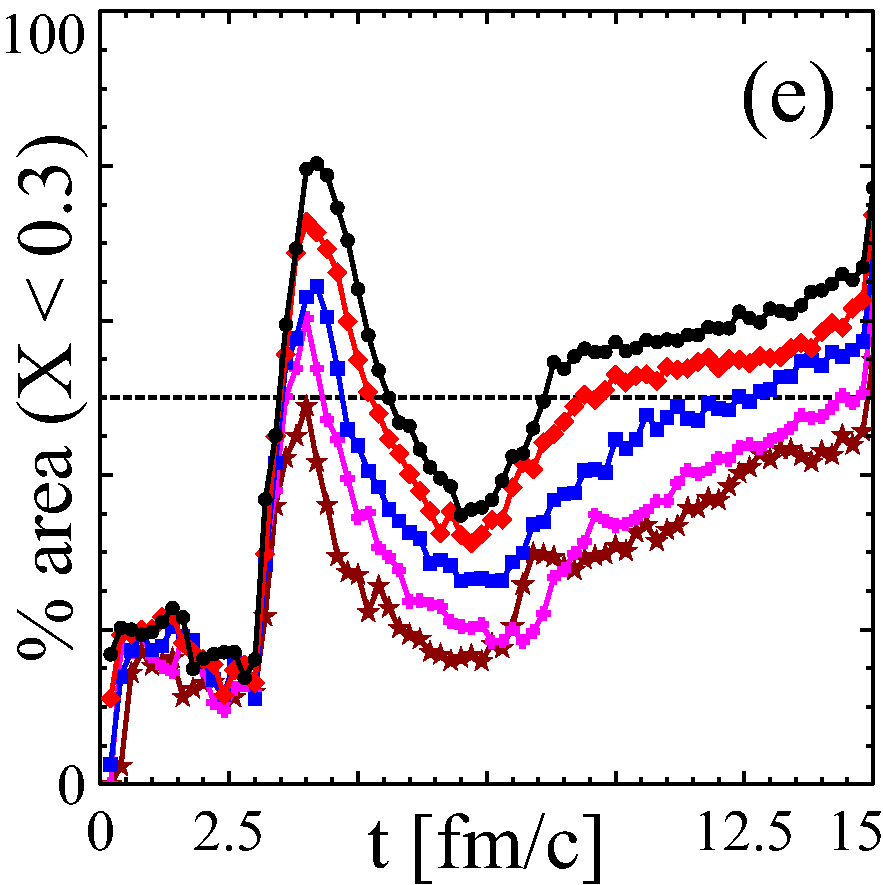
\includegraphics[width = 0.32\textwidth]{plots/thermalization_urqmd/plot_x_area_percentages_E80.pdf}
  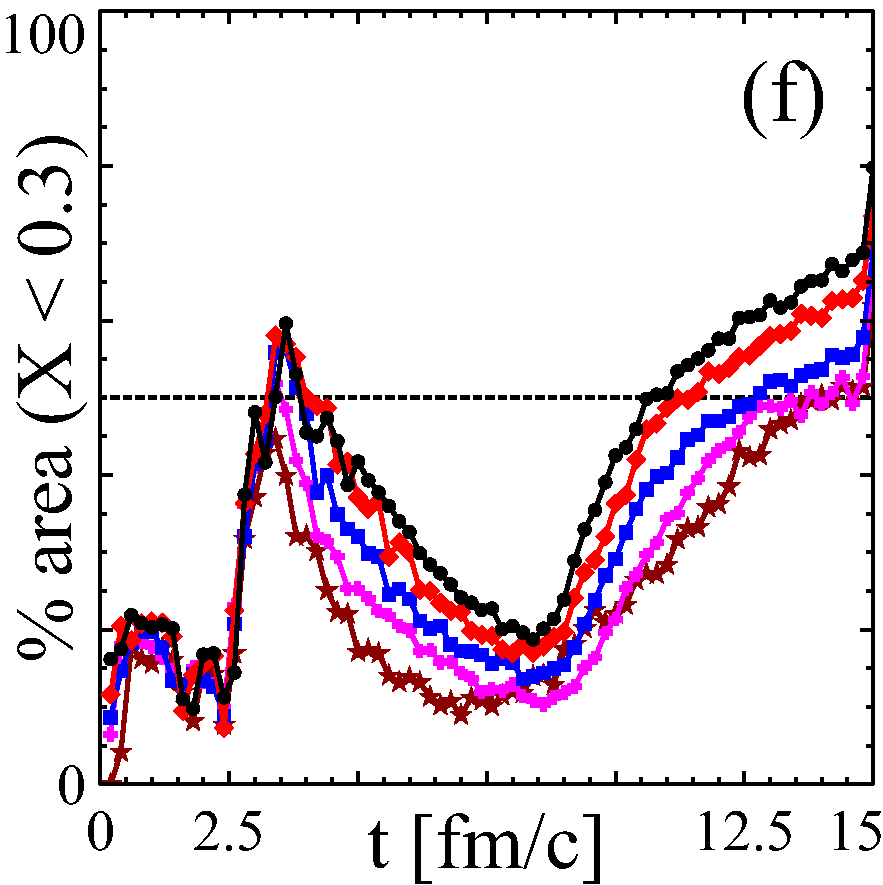
\includegraphics[width = 0.32\textwidth]{plots/thermalization_urqmd/plot_x_area_percentages_E160.pdf}
  \caption{Percentage of area in the event plane, where pressure anisotropy $X <
           0.3$, for Au+Au collision energies $\Elab = 5$, $10$, $20$, $40$, $80$,
           $160$ \emph{A} GeV (panels (a) - (f) correspondingly).}
  \label{FIG:x_area_percentages}
\end{figure}

After looking at the space-time evolution of the anisotropy in 2D as in
Fig.~\ref{FIG:x_paraview_space_time_evolution} for different energies, one gets
the impression that there is a special moment $t_{iso}$ for each energy and
centrality, before which pressures are highly anisotropic in the whole event
plane and after which there emerges a considerable isotropic region. To quantify
this feeling let us consider the ratio of the area, where $X < 0.3$ to the total area
versus time. From Fig.~\ref{FIG:x_area_percentages} one can see that there is
indeed a steep rise of the isotropized area at some point in time for every considered
energy and centrality. Let us define the \emph{isotropization time} $t_{iso}$
such that more than 50\% of the area has $X < 0.3$ at $t = t_{iso}$. The
behaviour of this isotropization time versus energy and centrality is compared
to the geometrical criterion in Fig.~\ref{FIG:t_x_energy}. One can see that the
isotropization time decreases with energy, but remains larger than the
geometrical criterion for all energies except $5\emph{A}$~GeV. It is interesting
to note that the isotropization time differs with centrality: for larger impact
parameters $b$ it slightly increases. One might assume that this has a pure
geometrical reason: $t_0 = 0$ is chosen in UrQMD as a moment when nuclei touch
each other in a central collision. However, for peripheral collisions the nuclei
will only touch at $t_0(b) = \frac{R}{\gamma v} (1 - \sqrt{1 - (b/2R)^2})$. In
Fig.~\ref{FIG:t_x_b} one can see that this naive expectation yields the right
trend: $t_{iso}$ rises with centrality and the rise is smaller for higher
energies. However, quantitatively it overestimates $t_{iso}$ for large impact
parameters.

\begin{figure}
  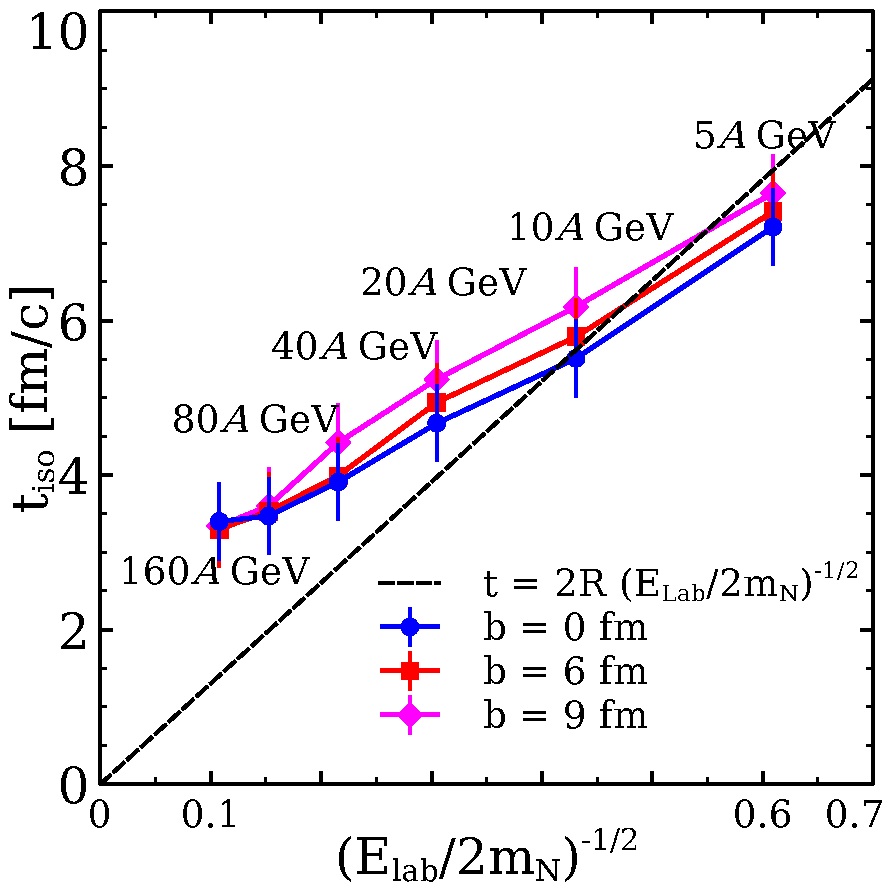
\includegraphics[width = 0.6\textwidth]{plots/thermalization_urqmd/t_x_vs_energy.pdf}
  \caption{Isotropization time $t_{iso}$ (see definition in the text) versus energy and centrality.}
  \label{FIG:t_x_energy}
\end{figure}

Let us compare the above findings to the study by Bravina et al.
\cite{Bravina:2008ra}, where one central cell of $(5 \times 5 \times 5)$ fm$^3$
was chosen to study the pressure anisotropy of the energy-momentum tensor in
Au+Au collisions. An isotropization time was  defined, and it did not change
significantly after zooming into the central cell to $(1 \times 1 \times 1)$ fm$^3$.
This allowed for the conclusion that isotropization happens rapidly in a large
volume. The isotropization time determined in this study also decreases with
collision energy. All of these results are confirmed in the present study.
However, our isotropization times are smaller than the ones obtained by Bravina
et al. There are two possible reasons for that.  First, the criterion for
isotropization used here is less strict: while here at least 50\% of
event plane area to have $X < 0.3$ is required, the central cell study demands
$p_z/p_x - 1 < 0.1$ in the whole cell, which corresponds to $X < 0.065$. Secondly,
here only the deviation of the energy-momentum tensor from equilibrium is considered,
but in the study \cite{Bravina:2008ra} also deviations of hadron multiplicities from
equilibrium are taken into account.

\begin{figure}
  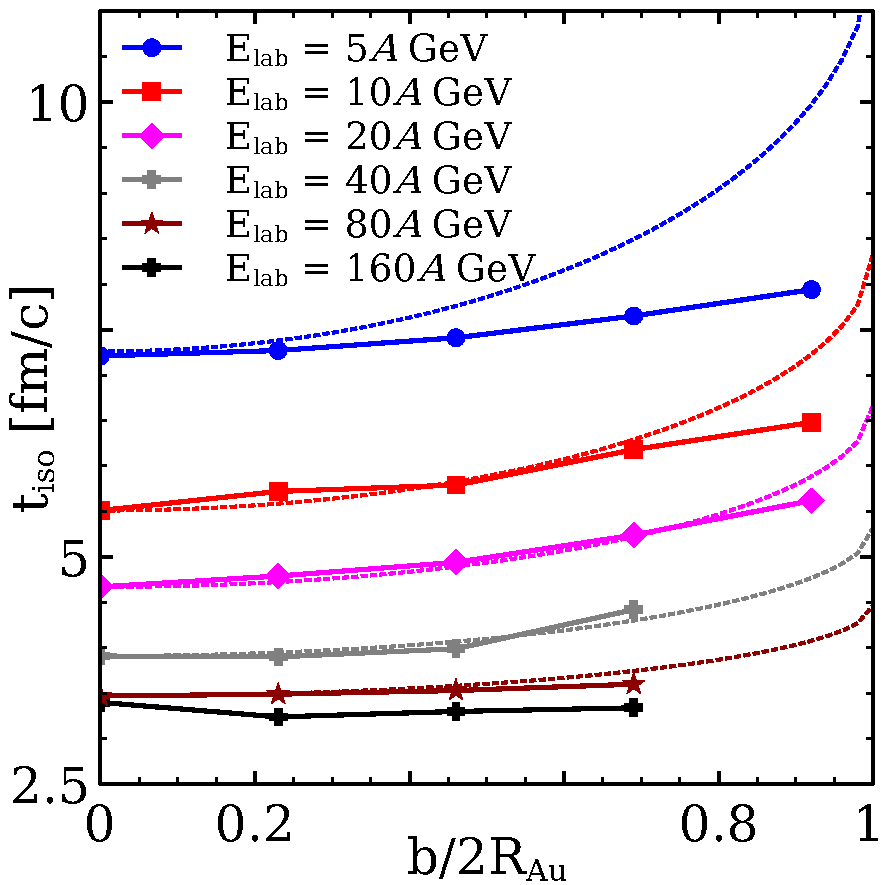
\includegraphics[width = 0.6\textwidth]{plots/thermalization_urqmd/t_x_vs_b.pdf}
  \caption{Isotropization time $t_{iso}$ (see definition in the text) versus
           centrality. The dotted lines represent the naive expectation from the
           collision geometry: $t_{iso}(b) = t_{iso}(b = 0) +
           \frac{R}{\gamma v} (1 - \sqrt{1 - (b/2R)^2})$.}
  \label{FIG:t_x_b}
\end{figure}

\subsection{Off-diagonality of $\Tmn$ in the local rest frame}

\begin{figure*}
  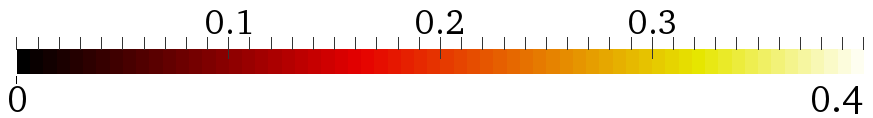
\includegraphics[height = 1cm]{plots/thermalization_urqmd/E80b6_x_paraview_color_legend.png} \\
  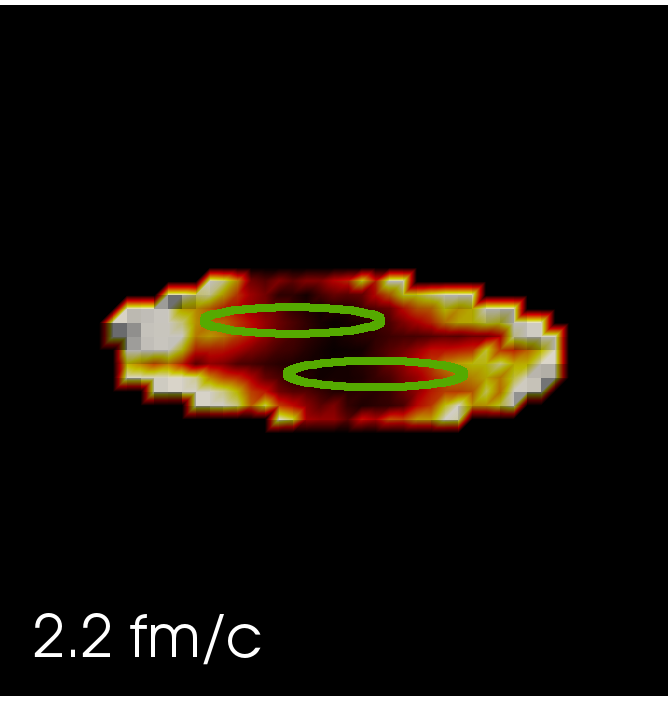
\includegraphics[width = 3.0cm]{plots/thermalization_urqmd/E80b6_y_paraview_t2_2fm.png}
  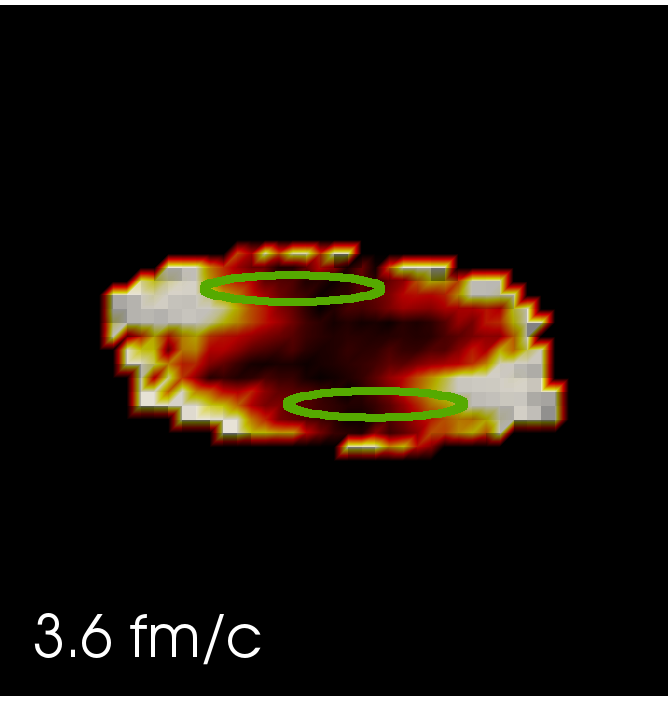
\includegraphics[width = 3.0cm]{plots/thermalization_urqmd/E80b6_y_paraview_t3_6fm.png}
  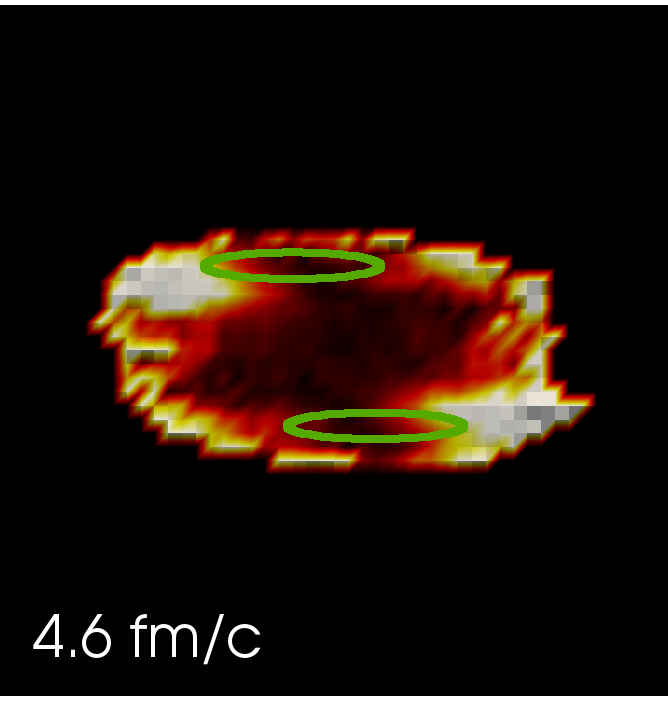
\includegraphics[width = 3.0cm]{plots/thermalization_urqmd/E80b6_y_paraview_t4_6fm.png}
  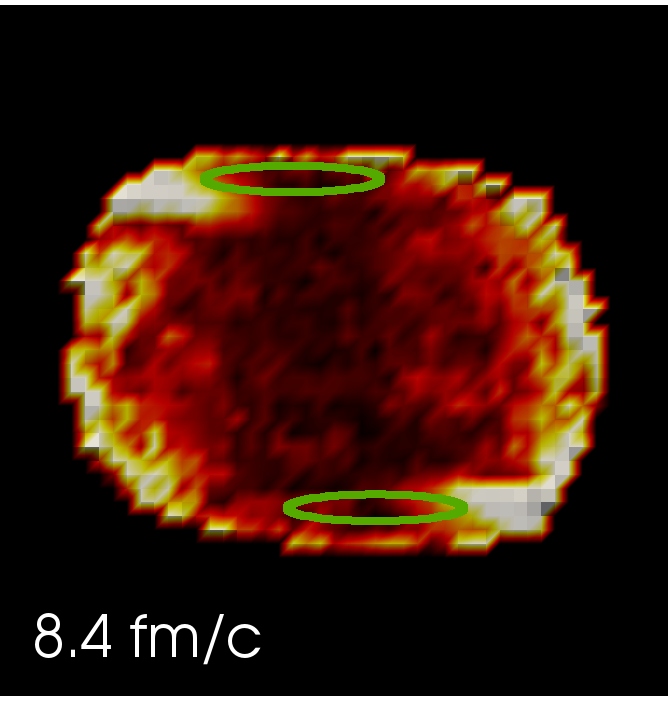
\includegraphics[width = 3.0cm]{plots/thermalization_urqmd/E80b6_y_paraview_t8_4fm.png}
  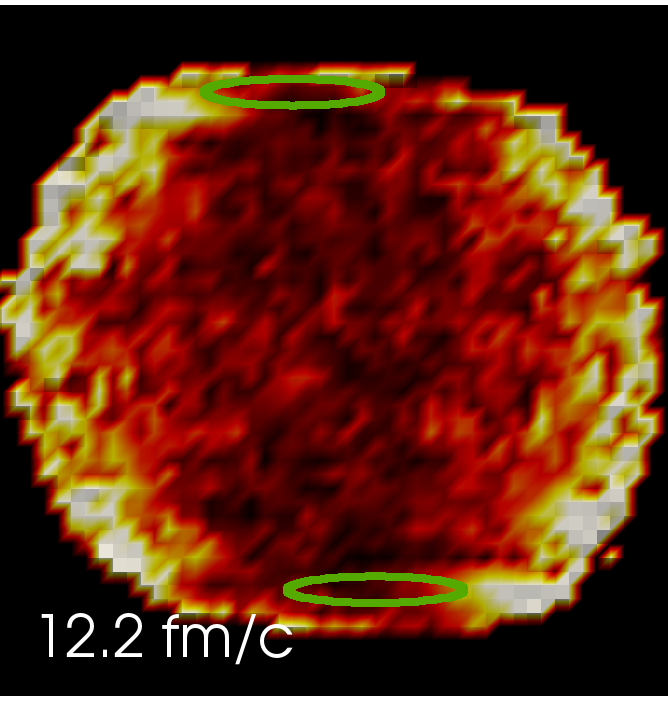
\includegraphics[width = 3.0cm]{plots/thermalization_urqmd/E80b6_y_paraview_t12_2fm.png}
  \caption{Space-time evolution of the off-diagonality $Y = \frac{3(|T^{12}_L| +
           |T^{23}_L| + |T^{13}_L|)}{T^{11}_L + T^{22}_L + T^{33}_L}$ (see color scale
           above the Fig.) for collision energy $\Elab = 80$ \emph{A} GeV and
           impact parameter $b = 6$ fm. If the value of $Y$ exceeds color map maximum,
           it is marked with the same color as maximum. Solid lines mark the positions
           of the nuclei, if they would not interact.}
  \label{FIG:y_paraview_space_time_evolution}
\end{figure*}

The off-diagonality $Y = \frac{3(|T^{12}_L| + |T^{23}_L| +
|T^{13}_L|)}{T^{11}_L + T^{22}_L + T^{33}_L}$ characterizes the size of the
off-diagonal components of the stress tensor compared to the pressure. In ideal
hydrodynamics $Y = 0$. For the applicability of viscous hydrodynamics it is
necessary that $Y \ll 1$. Here $Y_{crit} = 0.3$ is considered as a value, after which
viscous hydrodynamics is hardly applicable. An example for the space-time
evolution of $Y$ is given in Fig.~\ref{FIG:y_paraview_space_time_evolution}.
From this Fig. it can be seen that in the central region $Y$ is always small.
On the boundaries $Y$ is typically large due to statistical effects. A
quantitative study similar to the study of the pressure isotropy $X$ shows that
for all considered energies and centralities more than 80\% of the event plane
area have $Y < 0.3$ for the whole time of the evolution.

\subsection{Relative velocity between Landau and Eckart frames}


\begin{figure*}
  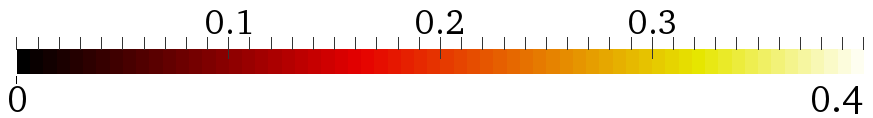
\includegraphics[height = 1cm]{plots/thermalization_urqmd/E80b6_x_paraview_color_legend.png} \\
  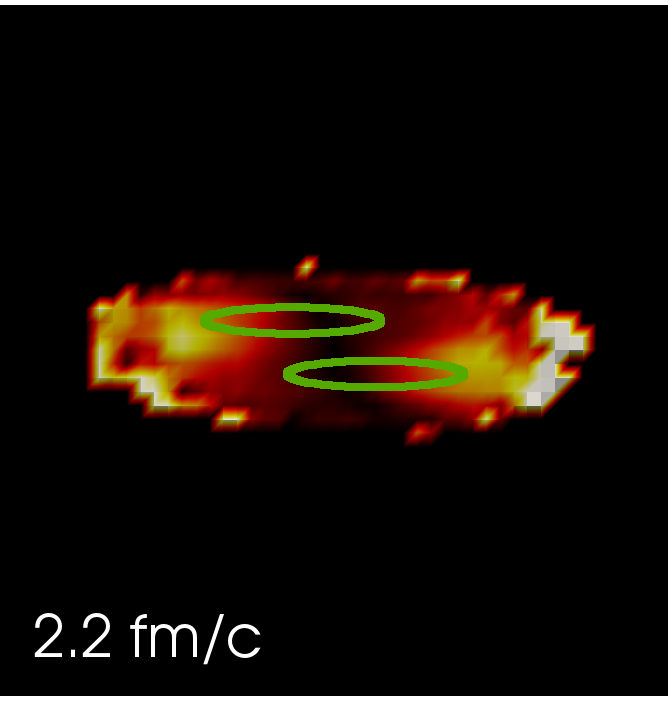
\includegraphics[width = 3.0cm]{plots/thermalization_urqmd/E80b6_vLE_paraview_t2_2fm.png}
  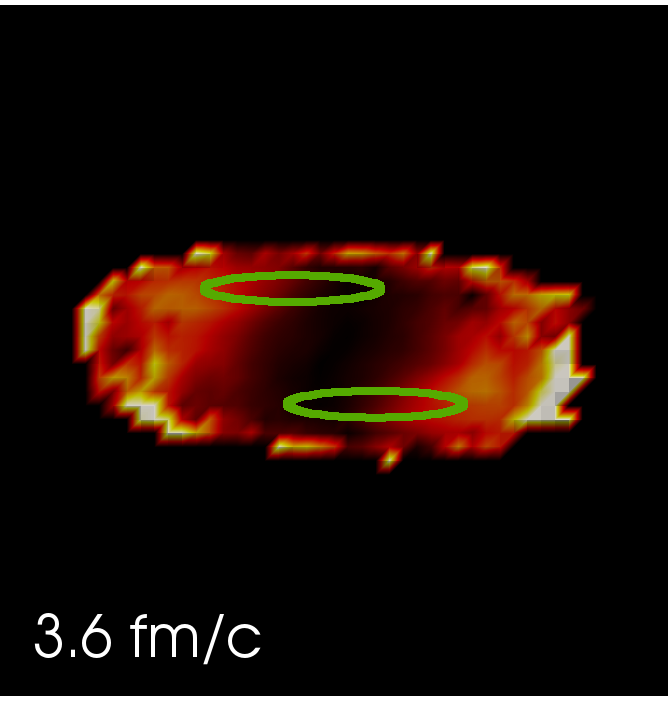
\includegraphics[width = 3.0cm]{plots/thermalization_urqmd/E80b6_vLE_paraview_t3_6fm.png}
  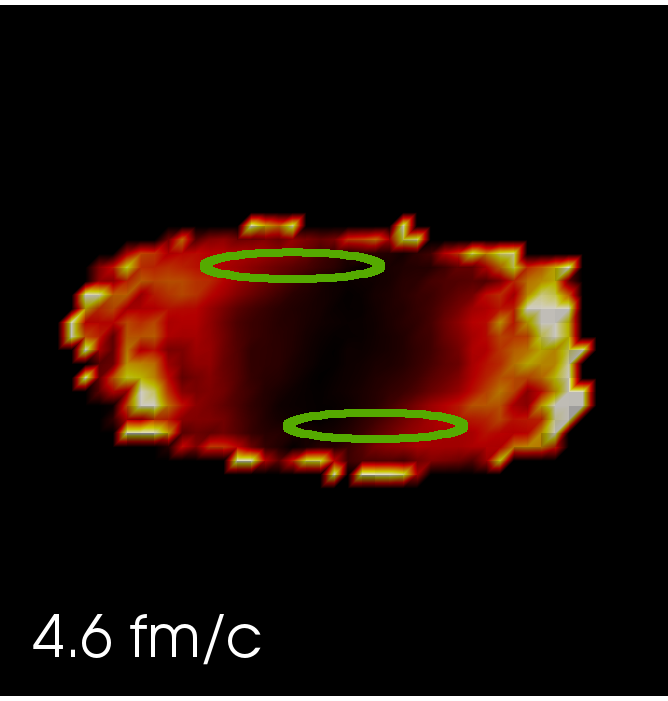
\includegraphics[width = 3.0cm]{plots/thermalization_urqmd/E80b6_vLE_paraview_t4_6fm.png}
  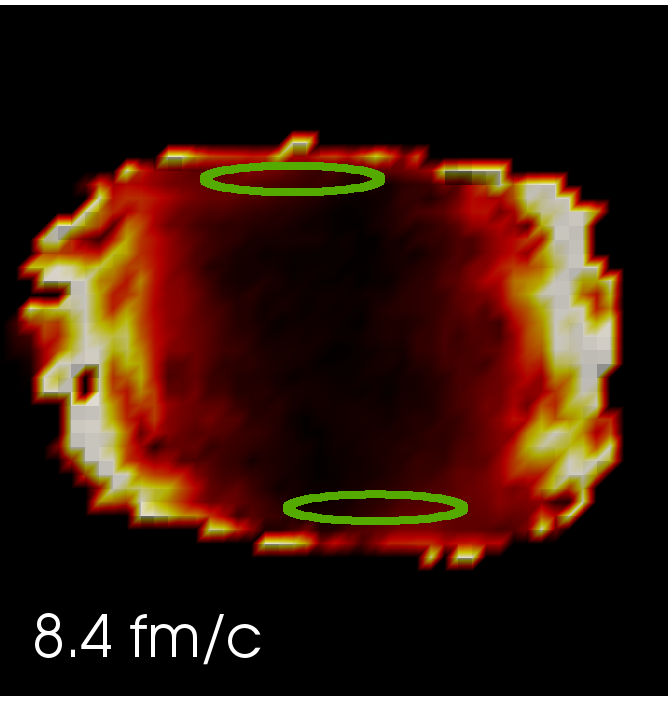
\includegraphics[width = 3.0cm]{plots/thermalization_urqmd/E80b6_vLE_paraview_t8_4fm.png}
  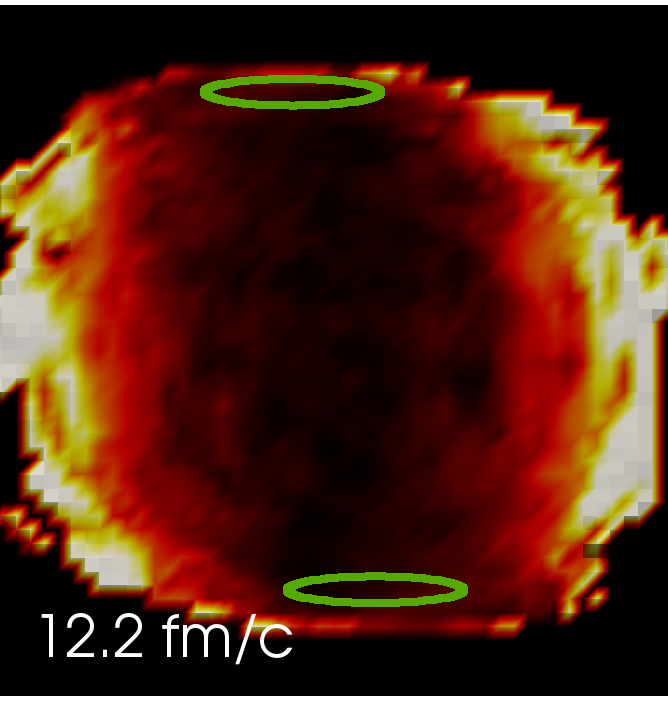
\includegraphics[width = 3.0cm]{plots/thermalization_urqmd/E80b6_vLE_paraview_t12_2fm.png}
  \caption{Space-time evolution of relative velocity between Landau and Eckart
           frames $v_{LE} = \sqrt{(j_L^1)^2 + (j_L^2)^2 + (j_L^3)^2}/j_L^0$ (see color
           scale above the Fig.) for collision energy in lab frame $E = 80\emph{A}$
           GeV, centrality $b = 6$ fm. If the value of $v_{LE}$ exceeds color map
           maximum, it is marked with the same color as maximum. Solid lines mark the
           positions of the nuclei, if they wouldn't interact.}
  \label{FIG:vLE_paraview_space_time_evolution}
\end{figure*}

The relative velocity between Landau and Eckart frames for the baryon charge
$v_{LE}$ is shown in Fig.~\ref{FIG:vLE_paraview_space_time_evolution}. At high
enough statistics the relative velocity between Eckart and Landau frames is not
an important factor. It is significant only on the borders of the system, where
the density is small and statistical effects play a role. But in all the rest of
the volume, for all the considered time evolution it remains small.

\subsection{The effect of momentum-space cuts}
\begin{figure}
  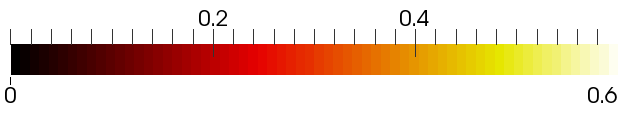
\includegraphics[height = 1cm]{plots/thermalization_urqmd/E80b6_x_paraview_color_legend_for_cuts.png} \\
  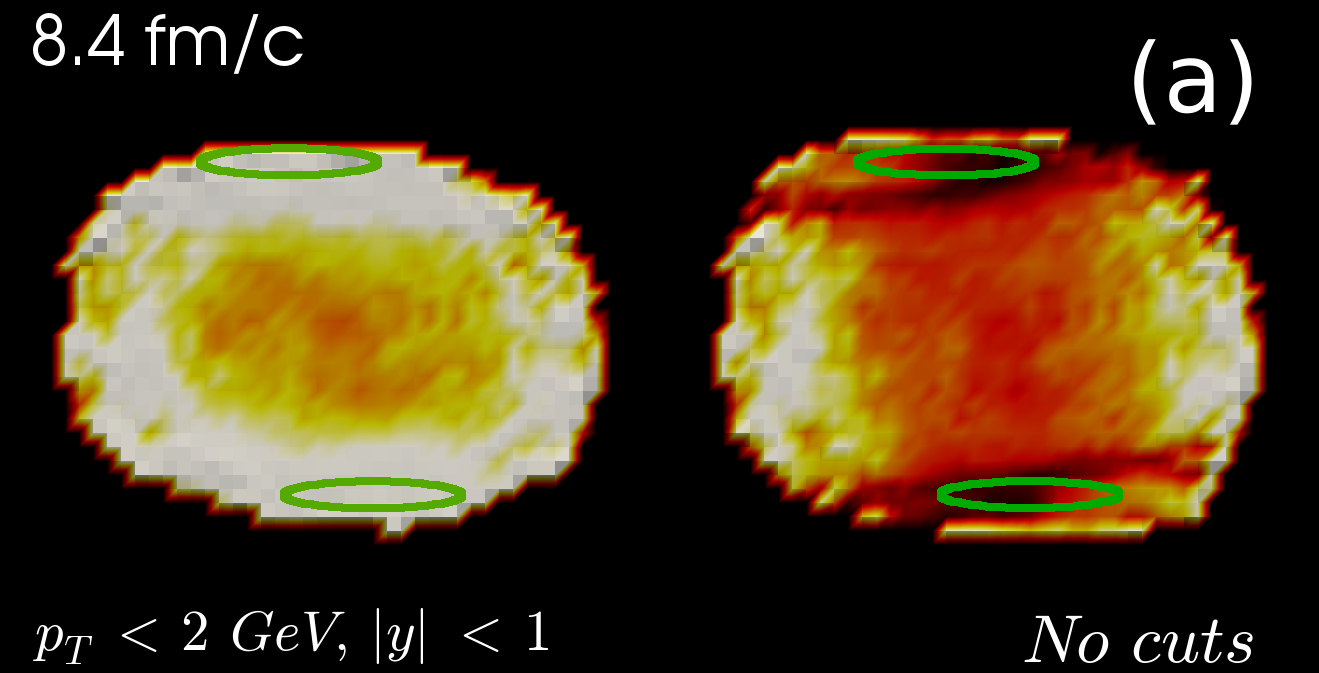
\includegraphics[width = 10cm]{plots/thermalization_urqmd/E80b6_x_paraview_cuts_comparison_t_8_4fm.png}
  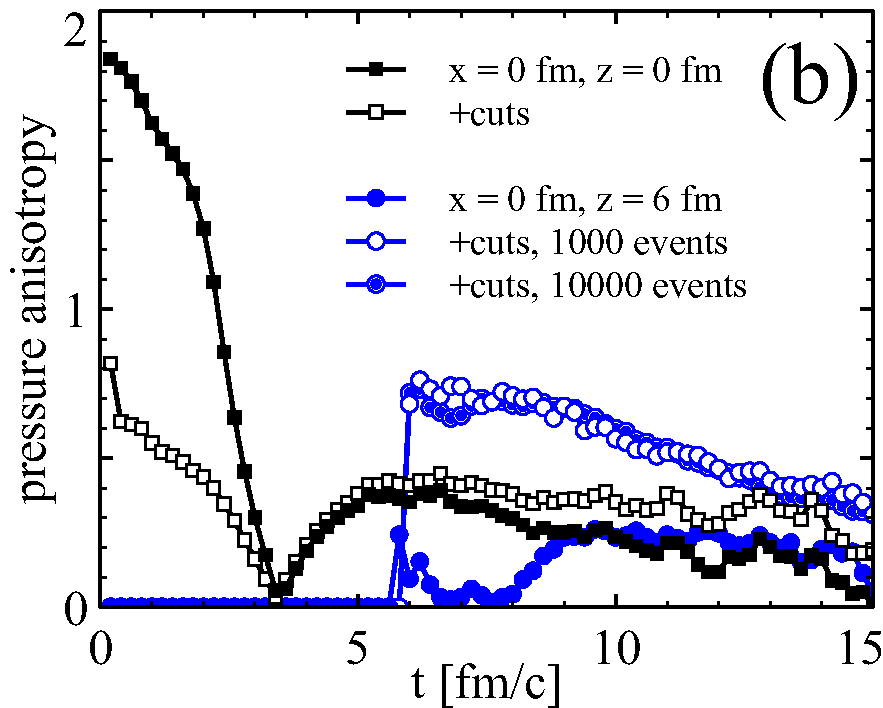
\includegraphics[width = 10cm]{plots/thermalization_urqmd/E80b6_x_vs_t_few_space_points_with_cuts.pdf}
   \caption{The effect of $p_T < 2$ GeV and $|y| < 1$ cuts on the space
            distribution of the pressure anisotropy $X =
            \frac{|T_L^{11}-T_L^{22}|+|T_L^{22}-T_L^{33}|+|T_L^{33}-T_L^{11}|}
            {T_L^{11}+T_L^{22}+T_L^{33}}$
            (see color scale above the Fig.) for collision energy 
            $\Elab = 80$ \emph{A} GeV and impact parameter $b = 6$ fm.
            If the value of $X$ exceeds color map maximum, it is marked with the same
            color as maximum. Solid lines mark the positions of the nuclei, if they
            would not interact.}
\label{FIG:X_paraview_cuts_effect}
\end{figure}

Previously, all participants were included into the $\Tmn$ calculation. However, it
is generally believed that soft particles at midrapidity thermalize faster,
therefore it might be insightful to impose cuts in momentum space, if one wants
to obtain a more isotropic $\Tmn$. On the other hand, applying transverse
momentum $p_T$ and rapidity $y$ cuts on a perfectly symmetric distribution
results in an asymmetry. In addition, these cuts decrease the statistics, which
leads to an increase of the anisotropy. To study the effect of the kinematic
cuts on the space distribution of the pressure anisotropy $X$, $\Tmn$ was
constructed only from particles with $p_T < 2$ GeV and $|y| < 1$ . The effect of cuts
on $X$ over space is shown in Fig. \ref{FIG:X_paraview_cuts_effect}. The statistical
effect does not play a significant role, because the results do not change after
increasing the number of events from $N_{ev} = 10^3$ to $10^4$. The large anisotropy
at very early times decreases after imposing cuts. But the anisotropy at later times
is strikingly larger with cuts, first of all in the regions behind the nuclei. While
without cuts it was possible to introduce an ''isotropization time'', when $X$ is
smaller than $0.3$ at more than 50\% of the area, with the cuts the anisotropy is so
high all over the space that the isotropization time cannot be introduced anymore.

\section{Summary and discussion}

The assumption of rapid equilibration was tested at $\Elab = $ = 5--160
\emph{A} GeV using the coarse-grained UrQMD transport approach.  The
energy-momentum tensor was studied locally in space and time and its deviation
from the ideal fluid form was quantified with two numbers: the pressure
anisotropy $X$ and the off-diagonality $Y$. First of all, it was shown that $X$
and $Y$ depend on the number of UrQMD events $N_{ev}$ used to construct $\Tmn$.
Low statistics implies large deviations, even if the underlying distribution
function is completely thermal and isotropic. An initial state constructed from
less than a few hundred events (or a few hundred testparticles equivalently) is
bound to deviate strongly from the ideal fluid form. The off-diagonality
appears to be mostly produced by this statistics effect. For large statistics
$Y$ tends to be small in all the collision region at all times. The pressure
anisotropy does not vanish with large statistics, it is a physical effect related
to the anisotropy of the underlying distribution function
$\mathit{f}(\vec{r},\vec{p})$. As a consequence, the initial state from UrQMD
with enough statistics is suitable for anisotropic hydrodynamics.

Unfortunately, all the results depend on the smearing parameter $\sigma$. With
larger $\sigma$ isotropization is reached later, but the degree of
isotropization is higher. From a practical point of view that means that
selecting large $\sigma$ one has to take larger fluidization time. This is in
agreement with conclusion of \cite{Petersen:2010zt} that a larger fluidization
time should be taken for larger $\sigma$ to obtain the same pion yield.
However, strictly speaking, the physical limit is $\sigma \to 0, \, \sigma^3
\rho N_{ev} \to \infty$. It was found that at small $\sigma$ the isotropization
time approaches the time of geometrical criterion $t_{geom} = 2R
(\Elab/2m_N)^{-1/2}$, so the rapid isotropization at the time of geometrical
overlap is partly justified, but only in the above mentioned limit. In the
existing models the smearing parameters and statistics are such that at
$t_{geom}$ the anisotropies are very high.

For the pressure anisotropy $X$ it was observed, that it exhibits a similar
pattern for all the considered collision energies and centralities: there is a
narrow interval of time, when it rapidly drops in a considerable volume. This
feature allowed us to introduce and study the isotropization time $t_{iso}$.
The time $t_{iso}$ can be considered as the time, when UrQMD starts to be
compatible with viscous hydrodynamics. At $t < t_{iso}$ the pressure anisotropy
$X$ is too high for viscous hydrodynamics to be applied. Isotropization time
decreases with collision energy, following the same trend as the geometrical
overlap time.  Based on this finding a new fluidization criterion is suggested:
$t_{iso} = t_{geom}(E) + \Delta t_0 (\sigma)$, where $\Delta t_0$ depends only
on the Gaussian smearing $\sigma$ and can be determined from
Fig.~\ref{FIG:t_iso_sensitivity_sigma}. A slight dependence of the isotropization
time on centrality was observed: it increases with impact parameter, but the
slope of this increase becomes smaller and smaller for higher energies. This
behaviour has a simple geometrical interpretation.
